\documentclass[letterpaper]{article}
\usepackage{aaai}
\usepackage{times}
\usepackage{helvet}
\usepackage{courier}

\usepackage{amsmath,amsfonts,amssymb,amsthm}
\usepackage{array}
\usepackage{amsmath,amssymb}
\usepackage[lofdepth,lotdepth]{subfig}
\usepackage{graphicx}
\usepackage{epstopdf}

%\usepackage{hyperref}
\frenchspacing

\newcommand{\link}{\mathit{link}}
\newcommand{\post}{\mathit{post}}
\newcommand{\photo}{\mathit{photo}}
\newcommand{\video}{\mathit{video}}
\newcommand{\all}{\mathit{all}}
\newcommand{\app}{\mathit{app}}

% place holder spacing hacks
\newcommand{\secmoveup}{\vspace{-1.2mm}}                %{\vspace{-0.12in}}
\newcommand{\bigsecmoveup}{\secmoveup\vspace{-.0mm}}   %{\vspace{-0.08in}}

\newcommand{\textmoveup}{\vspace{-0mm}}               %{\vspace{-0.08in}}
\newcommand{\bigtextmoveup}{\textmoveup\vspace{-0.0in}} %{\vspace{-0.06in}}
\newcommand{\itemmoveup}{\vspace{-0mm}}              %{\vspace{-0.04in}}
\newcommand{\eqmoveup}{\vspace{-0.0in}}                 %{\vspace{-0.16in}}
\newcommand{\captionmoveup}{\eqmoveup\vspace{-0.0in}}   %{\vspace{-0.16in}}
\newcommand{\refitemmoveup}{\vspace{-0mm}}            %{\vspace{-0.16in}}
% hold but hide chunks of text
\newcommand{\eat}[1]{}
\newcommand{\TODO}[1]{ {\color{blue}{\bf TODO:~{#1}}} }

%\newcommand{}{\mathit{}}
\newcommand{\x}{\mathbf{x}}
\newcommand{\dislike}{\mathit{dislike}}
\newcommand{\like}{\mathit{like}}
\newcommand{\likes}{\mathit{likes}}
\newcommand{\true}{\mathit{true}}
\newcommand{\false}{\mathit{false}}
\def\argmax{\operatornamewithlimits{arg\,max}}
\def\argmin{\operatornamewithlimits{arg\,min}}

\setcounter{secnumdepth}{0}

\begin{document}

\title{Social Affinity Filtering: Recommendation through \\Fine-grained Analysis of User Interactions and Activities}
\author{Anonymous}

\maketitle

\begin{abstract}
Content recommendation in social networks poses the complex problem of
learning user preferences from a rich set of avialable social information.
%and complex set of interactions (e.g., likes, comments and tags for posts, photos and videos) and
%activities (e.g., favourites, group memberships, page likes).  
While many social collaborative filtering approaches learn from aggregate statistics over the
social information, we propose a novel method, \textbf{\textit{social affinity filtering} (SAF)}, 
that take into account the fine-grained social interactions (e.g., likes, comments and tags for 
links, posts, photos and videos) and activites (eg, group memberships, page likes, favourites) 
information. We show that SAF yields higher accuracy than than a range of state-of-the-art 
(social) collaborative filtering approaches.
\eat{
we propose a different approach that leverages the fine grain-interactions(e.g., likes, comments and tags for links, posts, photos and videos) 
and activites(eg, group memberships, page likes, favourites)
: we first define
social affinity groups (SAGs) of a target user by analysing their
fine-grained interactions (e.g., likes, comments and tags for posts, photos and videos) 
and activities (e.g., group memberships, page likes, favourites).  Then we define Social 
affinity features based on SAGs and learn the target user's preferences
in a method we term \textbf{\textit{social affinity filtering} (SAF)}.}
%Then we learn which SAGs are most predictive of the target user's preferences
%in a method we term social affinity filtering (SAF).
Furthermore, we provide an analysis of informativeness of interactions and activity (based
on size). 
%We substantiate the advantage of learning via fine-grained social information than aggregate
%statistics by showing that some interactions and activities are more predictive than others.
Our analysis shows that some interactions and activities are relatively predictive than others which 
substantiate the essence and advantage of learning via fine-grained social information instead of
aggregate statistics.


%from recommender system which can be very crucial in building recommender system without
%much  . Our analysis shows that predictiveness varies over the directionality of interaction
%and videos interaction are highly predictive. Moreover, we found that small activities can 
%be highly predictive of user prefer


%We apply SAF to preference data from a set of Facebook users and their
%complete interactions with 38,000+ friends collected over a four month
%period.
%Our analysis demonstrates that SAF yields higher accuracy
%than a range of state-of-the-art (social) collaborative filtering approaches and that not all
%interactions and activities are equally predictive: among many insights, 
%we show certain user-to-user interactions are more
%informative than others  
%Our analysis demonstrates that SAF yields higher accuracy
%than a range of state-of-the-art (social) collaborative filtering approaches and 
%that not all interactions and activities are equally predictive: among many insights, 
%we show certain user-to-user interactions are more
%informative than others %(tagging is often more informative than
%commenting, video interactions are more informative than wall post
%interactions)
%we analyse trends in the relationship between the
%size of activity-based SAGs and informativeness
% (small groups can be
%highly informative while large groups are rarely informative).
%and we show that activity informativeness varies significantly with size.
%In summary, this work demonstrates the previously untapped
%features and the novel method of SAF to leverage them for
%state-of-the-art social recommender systems.


\end{abstract}

\section{Introduction}

%!TEX root = document.tex

\label{sec:introduction}

% motivate socical recommendation 
Online social networks such as Facebook record a very rich set of user
preferences  (likes of links, posts, photos, videos), user traits,
interactions and activities (conversation streams, tagging, group memberships,
interests, personal history and demographic data).  In the context of
 recent work on social recommendation~\cite{sorec,ste,lla}, and those on 
information diffusion %in social network analysis
~\cite{Goel2012structure,Romero2011hashtag,Bakshy2012chamber}, 
it is important to know which of these interactions or common traits
are actually reflective of common preferences.

Many recommendation methods for social networks 
use an aggregation approach to representing  
user interactions, such as performing 
low-rank factorization of the social relationships matrix~\cite{sorec} 
using a trust ensemble~\cite{ste},
or collapsing co-preferences and interactions as 
one indication of friend similarity~\cite{Noel2012NOF}.
The point of departure for this work, is the hypothesis that
fine-grained {\em affinities}, such as
different modalities of interaction (e.g. commenting vs tagging) 
and that different items relating to social preference 
(e.g. a university alumni group vs fans of a TV series) 
are of different importance for preference prediction.
Moreover, effective use of this information, i.e., {\em filtering}, 
will lead to better results in social recommendation.

To obtain quantitative answers to this question, 
we have built a Facebook App to collect a set of 
detailed user information and detailed interaction history 
available through the Facebook Graph API. 
We recommend links to each App user from the timeline of their 
friends and non-friends, and we record users' explicit likes 
and dislikes for the links being recommended to them. 
In this work, we explore the role of detailed user preferences 
and interactions for recommendation, called {\em social affinity filtering}.
% Our recent work~\cite{anonymous} designed new objective functions
%for social recommendation that out-perform state-of-the-art, 

In our 4-month interaction trace from 119 app users and their 38,000+ friends, 
we use detailed history of 22 different interaction types on users' timeline, 
along with their preferences on 3000+ groups, 4000+ favourites, and 10,000+ pages. 
%Do fine-grained social interactions help predict user preferences?
We found that social affinity filtering significantly 
outperforms state-of-the-art social recommendation, by up to 6\% in accuracy.
We also found that groups, pages, and favourites, 
as rich and active indications of user preference, outperforms interaction traces. 
Among the interactions, we found that those on videos are more predictive than those on other content types (photos, post, link), and that outgoing interactions (performed by the ego) 
is more predictive than incoming ones (performed by friends on the ego's timeline).
Among {\em groups}, {\em pages} and {\em favourites}, we found that the most  
predictive features have smaller membership size, and that favorite features corresponding to 
persistent activities (such as TV, books, activities) are more predictive than generic or 
temporally synchronized activities (such as interests, sports). 
These findings points to new directions for improving social recommendation, 
and open up interesting questions about the nature of interactions and social preferences. 

%\TODO{add table-of-content?}

%In this paper,
%we provide empirical answers for questions such as the following:
%\begin{itemize}
%%%lexing: make it sound a bit less technical and maintain the specificity, this is icwsm, hem
%%\item What is the probability that 
%\item How likely will a random user $u$ like
%photos that have been liked at least $k$ times by friends? 
%Or friends whose posts $u$ has commented on?
%%\item What is the probability that a random user $u$ will like any
%\item How likely will a random user $u$ like a
%link that is liked at least $k=2$ times by friends sharing common interests
%(movies, television, etc.), or sharing life history (same school or employer)? 
%What if the maximum number of friends sharing this interest is at most $n$?
%%\item What is the probability that a random male user $u$ 
%\item How likely will a male user $u$ like
%items liked at least $k=1$ times by his female friends?
%\end{itemize}

%While many of these queries may seem very narrow, we note that subtle
%changes in the query conditions and parameters above can lead to
%drastic swings in predictive probability.  For example, in the above
%queries, large variations in probability may be 
%observed by changing photo likes to post likes, changing
%wall comment interactions to photo comments, changing from $k=1$ to
%$k=2$ or $n=2$ to $n=4$, and changing the group definition from common
%school to common employer.

\eat{
To better understand these subtleties and to understand what
social interactions and user traits reflect common preferences on
Facebook, we proceed in the following sections to describe our data,
our experimental methodology, and various analyses according to our
methodology that shed light on the above questions. 
On one hand our observations confirm certain observations made previous 
on different networks, such as the diminishing returns of repeated exposures, 
on the other we also see a few new clues such as 
that very specific types of outgoing interactions are more predictive 
than other interactions. 
We then conclude with a summary of the key novel observations arising
from this study.
}


\section{Data Description}


We built a Facebook App\footnote{Name and link omitted
for anonymity.} to collect information about users, 
their interactions and preferences.  
%data about Facebook users and their Facebook friends
%are collected through our Facebook App. 
Our dataset contains information about each App user, along with a
subset of information about their friends visible to the App.  The
data collection is performed with full permission from the user and in
accordance with an approved Ethics Protocol\footnote{Link omitted for
anonymity.}.

Over 200 users installed the Facebook App sometime during the
evaluation period. At any time, around 100 users have actively used
the App. From these core App users, the App has access to their
detailed Facebook profiles and their interactions with a total of
39,850 friends.
%interaction data.  
While we have complete interaction data for the App
users with their friends, and profile data (including
wall post data) for the App users and friends, we do not have complete
interactions for the App users' friends (unless they themselves are
App users).  Hence in the forthcoming analysis, we limit our
evaluation to App users for which we are assured to have full
interaction data.

Our App tracks many user (and their friends') details and interactions
on Facebook.  Interactions that occur through wall posts provide a
rich variety of content and interaction data.  We distinguish four
Facebook items from wall posts: general posts (e.g., status updates,
activity updates such as new friends, and interactions such as the
user liked these pages), links, photos and videos. Four main
interactions on these items are permitted by Facebook: posting an item
to a friend's wall, commenting, liking, and tagging\footnote{Some
Facebook interaction features such as liking comments were introduced
after App user studies began and so are not tracked.}.  The App does
not track deletions of these items and interactions (e.g., unlike) for
performance reasons and we found very few deletions during an initial
testing stage.

%% Scott edited up to this point: please don't undo unless something
%% stated is incorrect.  We cannot use the name LinkR b/c it reveals
%% who we are.  I deleted some details of the ethics protocol as they
%% are not needed in this submitted version of the paper for review,
%% can add in camera-ready if needed.  Changed object -> item to be
%% consistent with later terminology.

%% Nguyen: please edit from this point on, only including statistics
%% that are relevant to data shown in the various plots, plus age
%% info as well (since this is useful to know).  So for example, 
%% you can comment out all non-gender, non-age demographics (locale, 
%% location, etc.) as well as unused table data (e.g., note that *only*
%% education and school -- first two rows of Table 3 are needed).
%% SVN has the record if we ever need to add this data back in.
%%
%% I did a search replace of LinkR with App... need to fix some 
%% awkward mentions.
%%
%% In short make sure all data mentioned is relevant to evaluation
%% section, other information is superfluous.

We summarize relevant basic statistics of the data in Table~\ref{tab:interactions}-\ref{tab:interests} below.
The tables distinguish the data from the App users and from
all App users and friends. Table~\ref{tab:interactions}
summarizes the number of records for each item (row) and interaction (column)
combination. Table~\ref{tab:demographics} shows 
some demographics from user profiles\footnote{Note that
count of schools are not unique as each user can attend more than one
degree of the same type.}.

\begin{table}
\centering
\begin{tabular}{|>{\small}l|>{\small}r|>{\small}r|>{\small}r|>{\small}r|}
\hline
\textbf{App Users} & \textbf{Posts} & \textbf{Tags} & \textbf{Comments} & \textbf{Likes} \\
\hline
\textbf{Wall} & 36,359 & 7,711 & 22,388 & 15,999 \\
\hline
\textbf{Link} & 5,304 & --- & 7,483 & 6,566 \\
\hline
\textbf{Photo} & 4,933 & 28,341 & 10,976 & 8,612 \\
\hline
\textbf{Video} & 245 & 2,525 & 1,970 & 843 \\
\hline
\hline
\textbf{App Users} & \textbf{Posts} & \textbf{Tags} & \textbf{Comments} & \textbf{Likes} \\
\textbf{and Friends} & & & & \\
\hline
\textbf{Wall} & 4,301,306 & 1,215,382 & 3,122,019 & 1,887,497 \\
\hline
\textbf{Link} & 678,612 & --- & 891,986 & 995,214 \\
\hline
\textbf{Photo} & 1,268,816 & 9,620,708 & 3,431,321 & 2,469,859 \\
\hline
\textbf{Video} & 59,244 & 904,604 & 486,677 & 332,619 \\
\hline
\end{tabular}
\caption{Number of records in Items and Interactions Tables. Rows are type of Facebook item and columns are type of Facebook interaction.}
\label{tab:interactions}
\end{table}


\begin{table}
\centering
\begin{tabular}{|>{\small}l|>{\small}r|>{\small}r|}
\hline
\textbf{Table} & \textbf{\#Records} & \textbf{\#Records} \\
& \textbf{(App Users)} & \textbf{(App User} \\
& & \textbf{and Friends)} \\
\hline
Users & 119 & 38,378 \\
\hline
\hline
\textbf{Column} & \textbf{\#Non-empty} & \textbf{\#Non-empty} \\
& \textbf{(App Users)} & \textbf{(App User} \\
& & \textbf{and Friends)} \\
\hline
Gender & 118 & 37,872 \\
%\hline
%Locale & 103 & 36,900 \\
%\hline
%Timezone & 103 & 117 \\
\hline
Birthday & 118 & 28,633 \\
%\hline
%Hometown\par Location & 63 & 17,584 \\
%\hline
%Current\par Location & 71 & 20,088 \\
\hline
\hline
\textbf{Breakdown} & \textbf{Count} & \textbf{Count} \\
& \textbf{(App Users)} & \textbf{(App User} \\
& & \textbf{and Friends)} \\
\hline
Male & 85 & 20,840 \\
\hline
Female & 33 & 17,032 \\
\hline
%High School & 104 & 29,503 \\
%\hline
%College & 115 & 29,223 \\
%\hline
%Graduate School & 56 & 7733 \\
%\hline
%%lexing: isn't it just "College" and not "Degree:College"
%Degree:\par High School & 104 & 29,503 \\
%\hline
%Degree:\par College & 115 & 29,223 \\
%\hline
%Degree:\par Graduate School & 56 & 7733 \\
%\hline
\end{tabular}
\caption{App user demographics.}
\label{tab:demographics}
\end{table}

\begin{table}
\centering
\begin{tabular}{|>{\small}l|>{\small}r|>{\small}r|}
\hline
\textbf{Table} & \textbf{\#Records} & \textbf{\#Records} \\
& \textbf{(App Users)} & \textbf{(App User} \\
& & \textbf{and Friends)} \\
%\hline
%Activities & 394 & 92,148 \\
%\hline
%Books & 266 & 52,690 \\
%\hline
%Favorite Athletes & 58 & 23,009 \\
%\hline
%Favorite Teams & 35 & 14,772 \\
\hline
Groups & 3,469 & 373,608 \\
\hline
Page Likes & 10,771 & 825,452 \\
\hline
Favourites & 4,284 & 892,820\\
%\hline
%Inspirational People & 39 & 7,815 \\
%\hline
%Interests & 153 & 36,085 \\
%\hline
%Movies & 616 & 149,197 \\
%\hline
%Music & 1,245 & 318,296 \\
%\hline
%Sports & 48 & 8,663 \\
%\hline
%Television & 819 & 144,308 \\
\hline
\end{tabular}
\caption{Groups of Interests Tables}
\label{tab:interests}
\end{table}

\begin{table}
\centering
\begin{tabular}{|>{\small}l|>{\small}r|>{\small}r|}\hline
&\textbf{Friend}  & \textbf{Non-Friend} \\
&\textbf{recommendation}  & \textbf{recommendation} \\
\hline
Like& 1392 & 1127 \\
\hline
Dislike& 895 & 2111\\
\hline
\end{tabular}
\end{table}


\section{Methodology}

%!TEX root = document.tex


As illustrated in Fig~\ref{fig:overview}, the high-level objective of this paper is to predict whether or not a user $u$ will like a digital item $i$ (in our test case, a link). 
We define user $u$'s preference for link $i$ as $like(u,i)$, this will be our prediction target. 
\begin{quote}
\begin{math}
likes(u,i) =  \begin{Bmatrix}
	  \true & \text{if user $u$ likes item $i$}\\
	  \false & \text{otherwise}
	  \end{Bmatrix}
\end{math}
\end{quote}

We define the social affinity between two users via their direct {\em interactions}
on various digital items, and their shared {\em activities} in different communities of the social network. 
We call our recommendation algorithm \textit{Social Affinity Filtering (SAF)}, as it infers 
$like(u,i)$ through the preference of their 
\textit{ Social Affinity Groups (SAG)}, i.e. a set of users with known preferences to link $i$, and who has at least one interaction or activity in common with $u$. 

\subsection{Action types on Facebook}
On Facebook, We use the term {\em Interactions} and {\em Activities} to refer to the range of user-user and user-community actions, respectively.

\noindent {\bf Interactions} describes the user-user communication in Facebook and can be defined in terms of modality, action and direction.
\begin{itemize}
\item \textbf{Modality:} (4 possibilities)
User $u$ can interact with another user $v$ via \textit{links, posts, photos} and \textit{videos} that appear in either user's timeline.

\item \textbf{Action type:} (3 possibilities)
%NOTE:- Actually link posted in facebook can be tagged in facebook. So its better not to mention that link
%cannot be tagged. I think its ok if we are not mentioning modality-action jointly in this short paper.
A user $u$ can \textit{comment} or \textit{like} 
user $v$'s item. He/she can also \textit{tag} user $v$ on an 
item, often indicating that user $v$ is present when the content is created(for photo/video)
or to explicitly raise user $v$'s attention for a post.

\item \textbf{Directionality:} (2 possibilities)
We look at \textit{incoming} and \textit{outgoing} interactions, i.e.,
if user $u$ comments on, tags, or likes user $v$'s item,
then this is an outgoing interactions for $u$, and an incoming interactions for $v$.
Although high correlation between \textit{incoming} and \textit{outgoing} interactions 
is recently observed~\cite{saez2011high}, whether or not interaction direction 
affects user preferences differently is still an open question we wish to answer
in this work. 
%then $u$ is in the set of incoming interactions for $v$
%and $v$ is in the set of outgoing interactions for $u$.
      								
\end{itemize}

%%%%%%%%%%%%%%%%%%%%%%%%%%%%%%%%%%%%%%%%%%%%%%%%%%%%%%%%%%%%%%
\begin{figure}[t!]
\centering
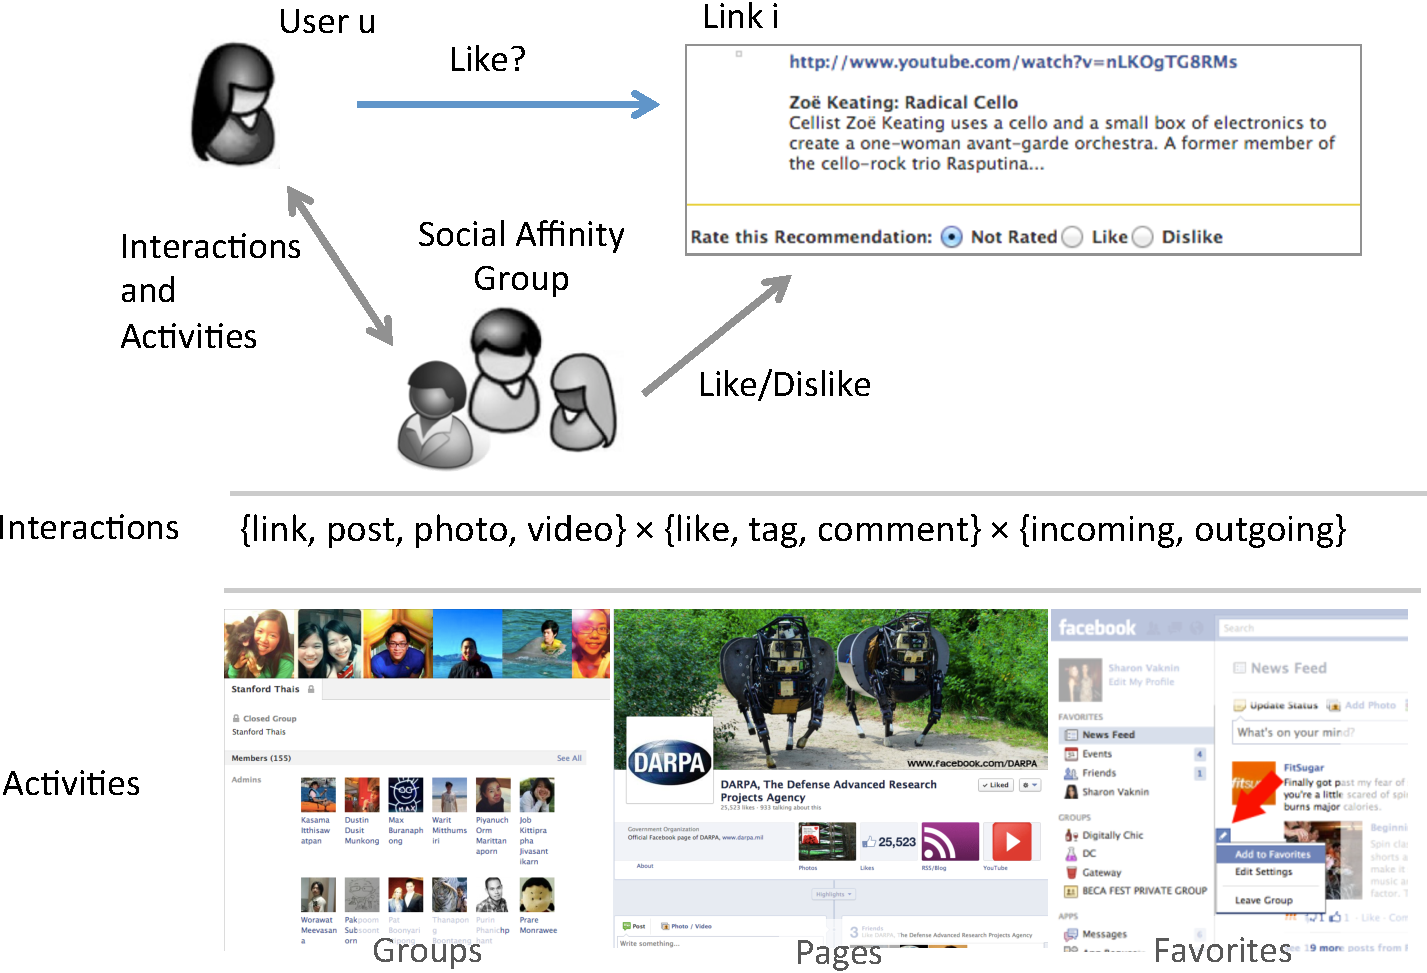
\includegraphics[width=1\linewidth,height=50mm]{data/overview}
\caption{Overview of social affinity for link recommendation.
A \emph{social affinity group (SAG)} consists of the set of alters 
of a user $u$ (ego) who have a
certain interaction or share an activity membership with $u$.
Alters defined by SAGs serve as proxies for an ego's interest with some
SAGs showing stronger affinity with an ego as learned by \emph{social affinity filtering (SAF)}
and analysed subsequently.}
\label{fig:overview}
\end{figure}
%%%%%%%%%%%%%%%%%%%%%%%%%%%%%%%%%%%%%%%%%%%%%%%%%%%%%%%%%%%%%%

%There are a total of 22 interaction types. Namely the cross-product of modalities, actions and directions, minus {\em link-tag-\{incoming, outgoing\}} since links cannot be tagged in Facebook.

%\subsection{Activities}
%\noindent
% Can we insert more specific links to Facebook blog?  -SPS


{\bf Activities} describes the user interactions with Facebook communities like groups, pages, favourites.
\begin{itemize}
  %@SCOTT/LEXING following defination are taken from facebook blog. I am confused how to cite it %
\item \textbf{Groups} on Facebook 
% I didnt find facebook favourites defination in facebook blog - Suvash
\footnote{Facebook Blog (Groups/Pages): \surl{http://www.facebook.com/blog/blog.php?post=324706977130}
%\footnote{From Facebook Blog: 
%\surl{http://www.facebook.com/blog/blog.php?post=324706977130}, ``Groups are the place for small group communication and for people to share their common interests and express their opinion. Groups allow people to come together around a common cause, issue or activity to organize, express objectives, discuss issues, post photos and share related content''. 
\label{fn:fbblog}}
are analogous to community organizations in the real-world. It allows users to declare membership and supports people to organize activities, to post related content, and to have recurring discussions about them.  Examples of groups include {\em Stanford Thai} (Fig~\ref{fig:overview} bottom left), or {\em Harvard Debate Club}.
\item \textbf{Pages} on Facebook \textsuperscript{\ref{fn:fbblog}}
  %\footnote{Facebook Blog (Pages): \surl{http://www.facebook.com/blog/blog.php?post=324706977130}}
 % \footnote{From Facebook Blog: 
%(\surl{http://www.facebook.com/blog/blog.php?post=324706977130} ``Facebook Pages enable public figures, businesses, organizations and other entities to create an authentic and public presence on Facebook. Facebook Pages are visible to everyone on the internet by default. Facebook user can connect with these Pages by becoming a fan and then receive their updates and interact with them.'' }
  %\footnotemark[\ref{fn:fbblog}] 
  are analogous to the homepages of people, organizations and events on the world-wide-web. They are publicly visible, and users can subscribe to the updates on the page, and also engage in discussions. Example pages include {\em DARPA} (an organization, Fig~\ref{fig:overview} bottom middle), or {\em Beyonce} (a singer).
\item \textbf{Favourites}  
\footnote{Facebook Blog (Favourites): \surl{https://www.facebook.com/help/232262810142682}} 
are analogous to bookmarks. It is a user-created list containing various digital items such as Facebook apps, books, music etc. indicating their interest. Example favourite items include {\em Big Bang Theory} (TV series), or {\em FC Barcelona} (soccer club). Fig~\ref{fig:overview} bottom right show a Facebook screenshot when a user adds a favourite.
 %\footnote{According to Facebook Blog, (\surl{https://www.facebook.com/help/232262810142682} ``Facebook facilitates a wide variety of user selected favourites (Activities, Favorite Athletes, Books, Interests, Movies, Music, Sports, Favorite Teams, Television). These favourites allow a user to associate themselves with other people who share their same favourite tendencies.}
\end{itemize} 

Our evaluation includes 3000+ {\em group}, 4000+ {\em page} and 10,000+ {\em favourite} 
features as detailed in Sec~\ref{sec:datadesc}.

%% This is good text, but probably better in related work.  We have CIKM reviewers here who are
%% just skimming and trying to follow the technical setup in the initial sections... this
%% serves as a bit of a digression that detracts from some of the more important quantitative
%% points that we want to drive home with the reader as early as possible.  -SPS
\eat{
Note that the notion of affinity we adopt is based on direct user {\em actions}, rather than
static profile information, or structural information of the social graph. 
We believe this is a useful view into the social network, as it was recently pointed out
that a user's attention (i.e., interactions) are divided among a small subset of Facebook friends~\cite{backstrom2011center}, and that ratings of real-world friendship strength seems to be more predictable from the intimacy, intensity, and duration of interactions, than from social distance and structural information~\cite{gilbert2009predicting}. Our affinity definition is based on direct interactions within a users' ego network, this is complementary to 
a recent alternative~\cite{Panigrahy2012ubr} that uses number of paths between two users encodes the resilience of network structure, 
as it was recently found~\cite{Goel2012structure} that the vast majority of information diffusion
happens within one step from the source node. }
% interactions
%Our affinity
%\cite{Wilson2012BSG}


\subsection{Social Affinity Groups}
\label{ssec:sag}

\eat{
The major objective of this paper is to evaluate the effectiveness of \textit{Social Affinity Filtering (SAF)} and fine grained 
analysis of the informativeness of Interactions and Activities.We divide our recommendation algorithm into two categories based 
on Interactions and Activities of 
}

Based on the definitions of {\em interaction}  and {\em activities} above, 
%\textit{ Social Affinity Groups (SAG)} with target item, 
we define two types of {\em social affinity groups} of a user with a target item,
namely \textit{Interaction  Social Affinity Groups (ISAG)} and \textit{Activity Social Affinity Groups (ASAG)}.

\begin{itemize}
  \item \textbf{Interaction  Social Affinity Groups}. First we define, interaction affinity classes as cartesian-product of 
  Interaction modality, action and direction.
  %\begin{quote}
  \begin{align*}
  	\textit{Interaction Affinity Classes} := \, & \{\link, \post, \photo, \video\} \\
                                                & \times \{\like, \ttag, \comment\} \\
                                                & \times \{\incoming, \outgoing\}
  \end{align*}
  %\end{quote}
  %Additionally, we add friendship interaction affinity class. \\
  We define,\\
  \textit{ISAG(u, k)} $:=$ \textit{the set of the users who have interaction $k$ with user $u$}.\\
   For example,
   %\begin{quote}
   \textit{ISAG(u, link-like-incoming)}  is a set of users who have liked link posted by user $u$.
   %\\
   %\textit{ISAG(u, photo-comment-outgoing)} is the set of all users whose photos received at least one comment from $u$.
   %\end{quote}
\item \textbf{Activity Social Affinity Groups}: We define activity social affinity groups based on group membership, page likes and user favourites.\\ \\
	\textit{ASAG(u, k)} $:=$
							\begin{math} 
							\begin{Bmatrix}
								members(k) & if\ u \in members(k)\\ 	
								\varnothing & otherwise
							\end{Bmatrix}
							\end{math}
	where, 	\textit{members(k)} $:=$ set of users who joined/liked/favourited activity k.		
	%\begin{quote}
	%\textit{ASAG(u, k)} $:=$ the set of the users who have common preference for entity $k$ (group, page, favourite) with user $u$.   
	%\end{quote}
\end{itemize}


\subsection{Social Affinity Features}
\label{ssec:SAfeature}
We define Interaction and Activity affinity features for target user $u$ and item $i$ for defined SAGs $ \langle X_{1},X_{2}\ldots,X_{k}\rangle$ as
  %\begin{quote}
  \begin{equation*}
   X_{k,u,i} = \begin{Bmatrix}
   		\mathit{1} & \text{if}\ \exists v\in SAG(u,k) \wedge likes(v,i)\\ \\
   		\mathit{0} & \text{otherwise}
   \end{Bmatrix}
  \end{equation*}

SAG corresponds to ISAG and ASAG for Interaction and Activity features respectively. Furthermore, we add extra friend feature for interaction which encodes whether the target item $i$ is liked by friend or not.

% \begin{itemize}
%   \item   
%   \item \textbf{Interaction Social Affinity Features} : We define Interaction affinity features for target user $u$ and item $i$ for ISAG's classes 
%   $ \langle X_{1},X_{2}\ldots,X_{k}\rangle$ as
%   %\begin{quote}
%   \begin{equation*}
%    X_{k,u,i} = \begin{Bmatrix}
%    		\mathit{true} & \text{if}\ \exists v\in ISAG(u,k) \wedge likes(v,i)\\ \\
%    		\mathit{false} & \text{otherwise}
%    \end{Bmatrix}
%   \end{equation*}
%   %\end{quote}
%   Additionally we add friend feature which encodes whether the target item $i$ is liked by friend or not.
%   \item \textbf{Activity Social Affinity Features} : We define activity affinity features for target user $u$ and item $i$   \
%   $ \langle X_{1},X_{2}\ldots,X_{k}\rangle$ as\\ \\
%   \begin{equation*}
%    X_{k,u,i} = \begin{Bmatrix}
%    		\mathit{true} & if\ \exists\ v\in \ ASAG(u,k) \wedge likes(v,i)\\ \\
%    		\mathit{false} & otherwise
%    \end{Bmatrix}
%   \end{equation*}
% 	In our analysis we use only those features (groups, pages and favourites) that are joined/liked by at least one of our app users.
% \end{itemize}

\eat{
%% SCOTT already covered these elsewhere
%% Hmmm... maybe I forgot to :)  -SPS
We train naive bayes, Logistic Regression(LR) and Support Vector Machine(SVM) model with affinity features.
Logistic Regression and SVM algorithm was implemented using \textit{LIBLINER} \cite{liblinear} package. 
We define Constant predictor as baseline predictor. Constant predictor predicts the most common outcome in our datase ie disliket.
We compare the performance of Social Affinity Filtering with the state of the art social collaborative filtering technique 
Social MatchBox(SMB)\cite{SMB}.

In real world social networks activity features grows very quickly as number of user in social network increases. This motivates the fine grained
analysis of informativeness of social affinity features. Furthermore, fine grained analysis of interactions helps to understand the nature of user-user 
interactions and its predictiveness in greater detail. Hence, for the analysis of activities and interactions we rank the features using
\textit{Conditional Entropy}. 
\textit{Conditional Entropy} is defined as
\begin{quote}
\begin{math}
H(Y|X=\true) = \\-\sum_{y\in{(like,dislike)}} p(y|X$=$true)$ $log( p(y|X$=$true))
\end{math}
\end{quote}

With the data and methodology now defined including all dimensions of our analysis, we now proceed to an in-depth discussion of our findings.
}




 






%\section{Evaluation}

%\begin{itemize}
  \item Page likes are most predictive followed by group and favourites
  \item Mutual information vs Size plot shows that the most predictive groups/page/favourites are spread around middle. This signifies that medium sized groups/pages/favourites are more predictive (!!!although not very strong signal)
  \item Collapsed mutual information ranking \\Video $>$ Photo $>$ Post $>$ Link\\ Comments $>$ Like $>$ Tags\\
   (No significant difference between Incoming and Outgoing)
   \item For Large social networks encoding user's membership(group/pages/favourites) as features and performing matrix factorization is not scalable (as there are millions of groups/pages/activities). This research shows that the memebership can be directly plugged into existing highly scalable algorithms to achieve better accuracy than state of art matrix factorization techniques. 
\end{itemize}


\begin{figure}
\centering
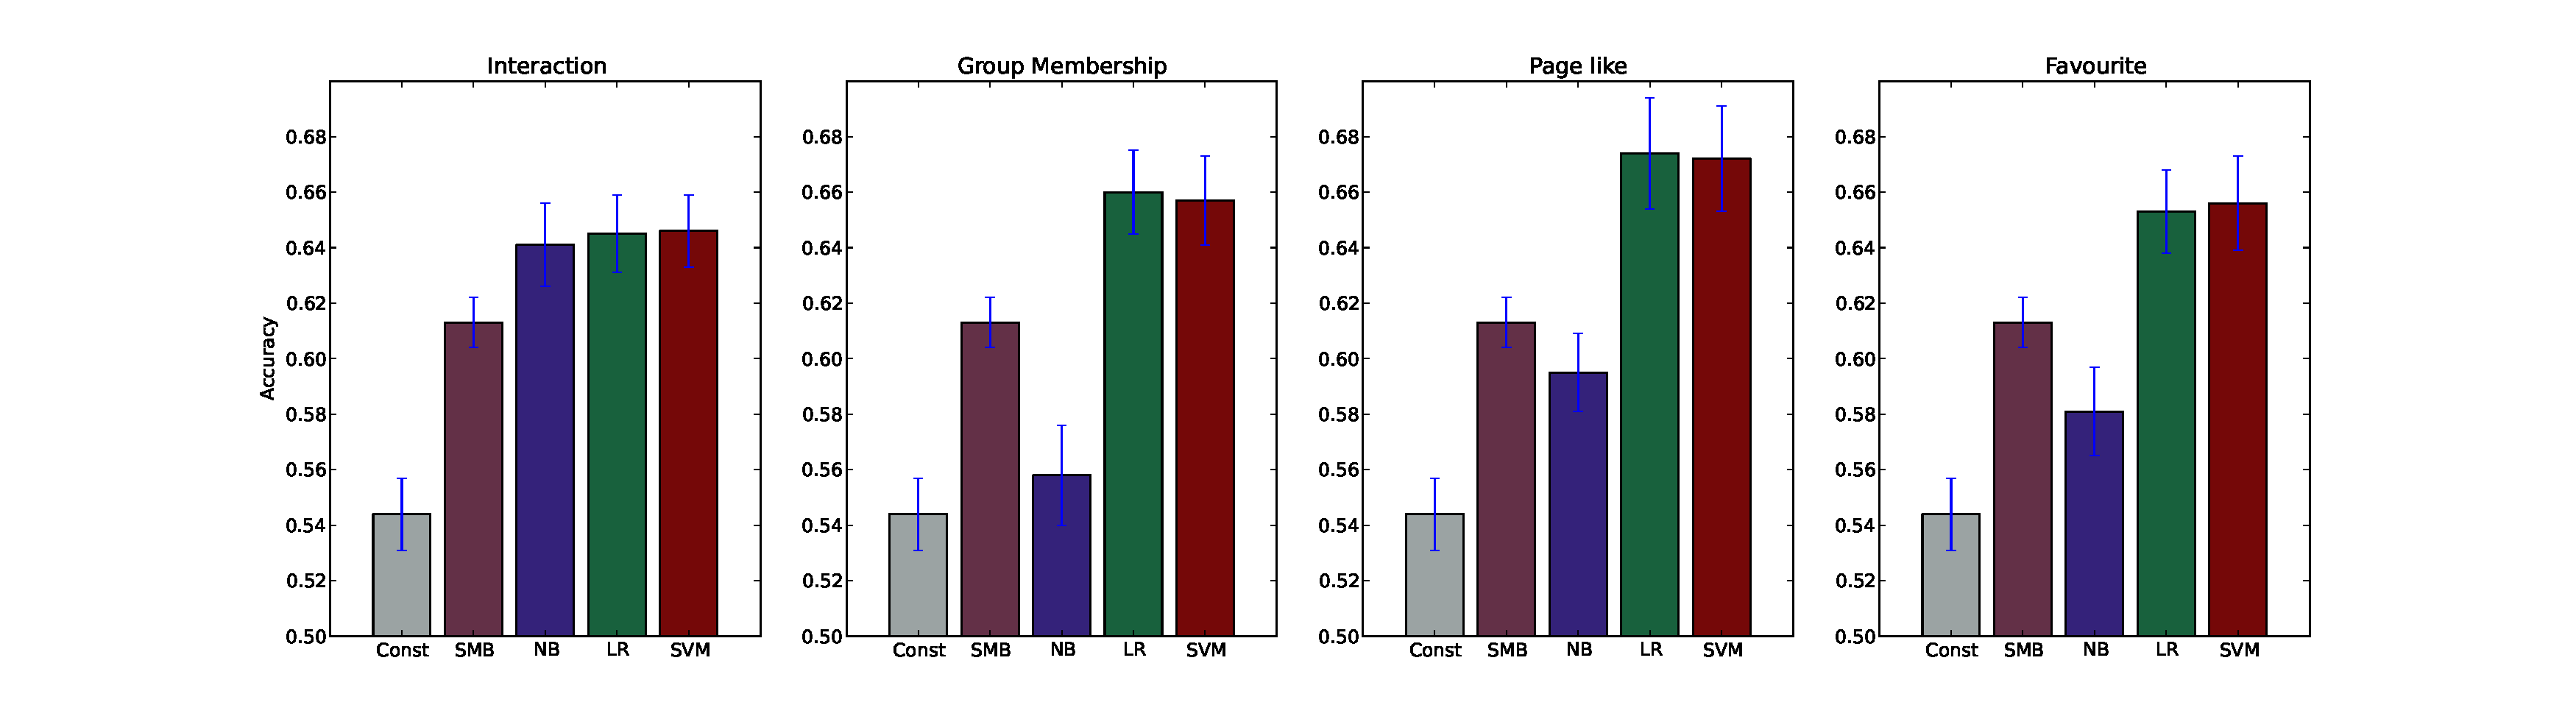
\includegraphics[scale=0.25]{data/accuracy.eps}
\caption{Accuracy plots}
\label{Fig: Accuracy}
\end{figure}

\begin{figure}
\centering
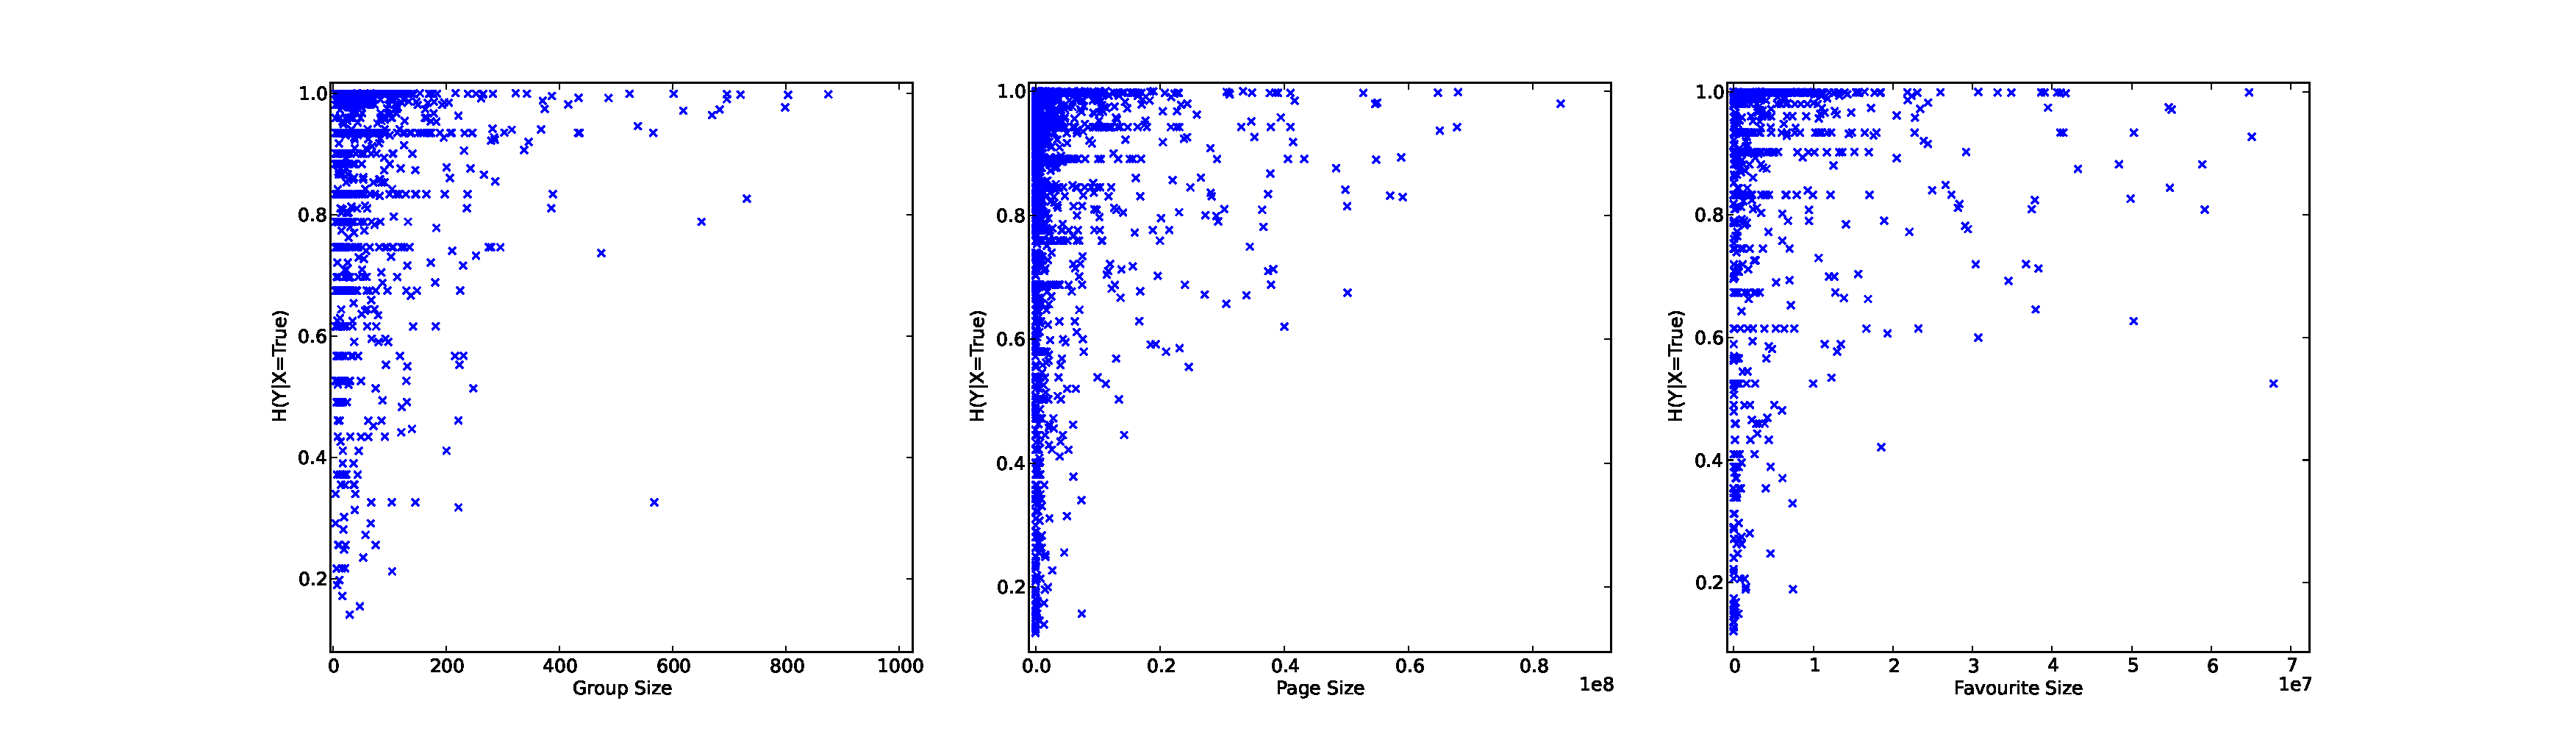
\includegraphics[width=100mm, height=30mm]{data/CEvsSize.eps}
\caption{Conditional Entropy vs Size}
\label{Fig: Conditional Entropy vs Size}
\end{figure}

\begin{figure}
\centering
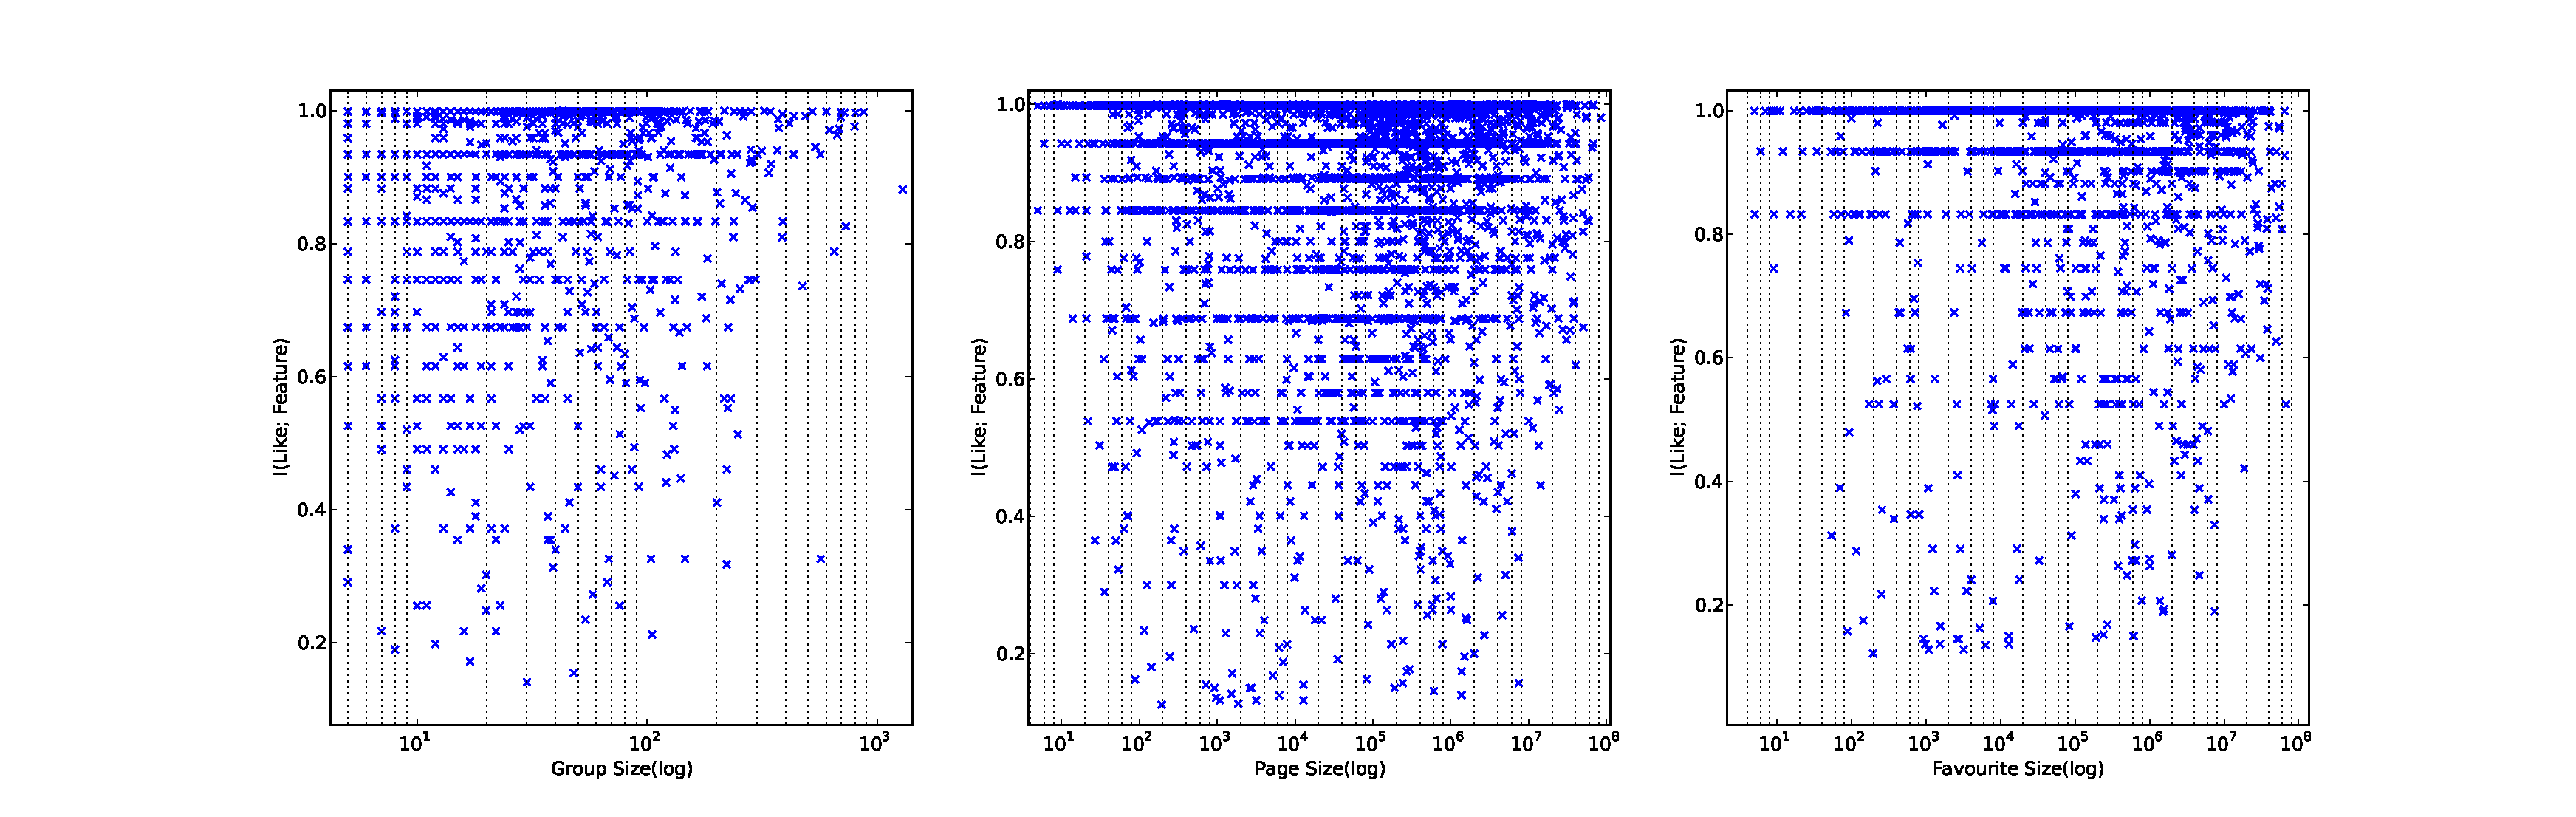
\includegraphics[width=100mm, height=30mm]{data/CEvsSizeLog.eps}
\caption{Conditional Entropy vs Size(log)}
\label{Fig: Conditional Entropy vs Size(Log)}
\end{figure}

\pagebreak


\begin{figure}
\centering
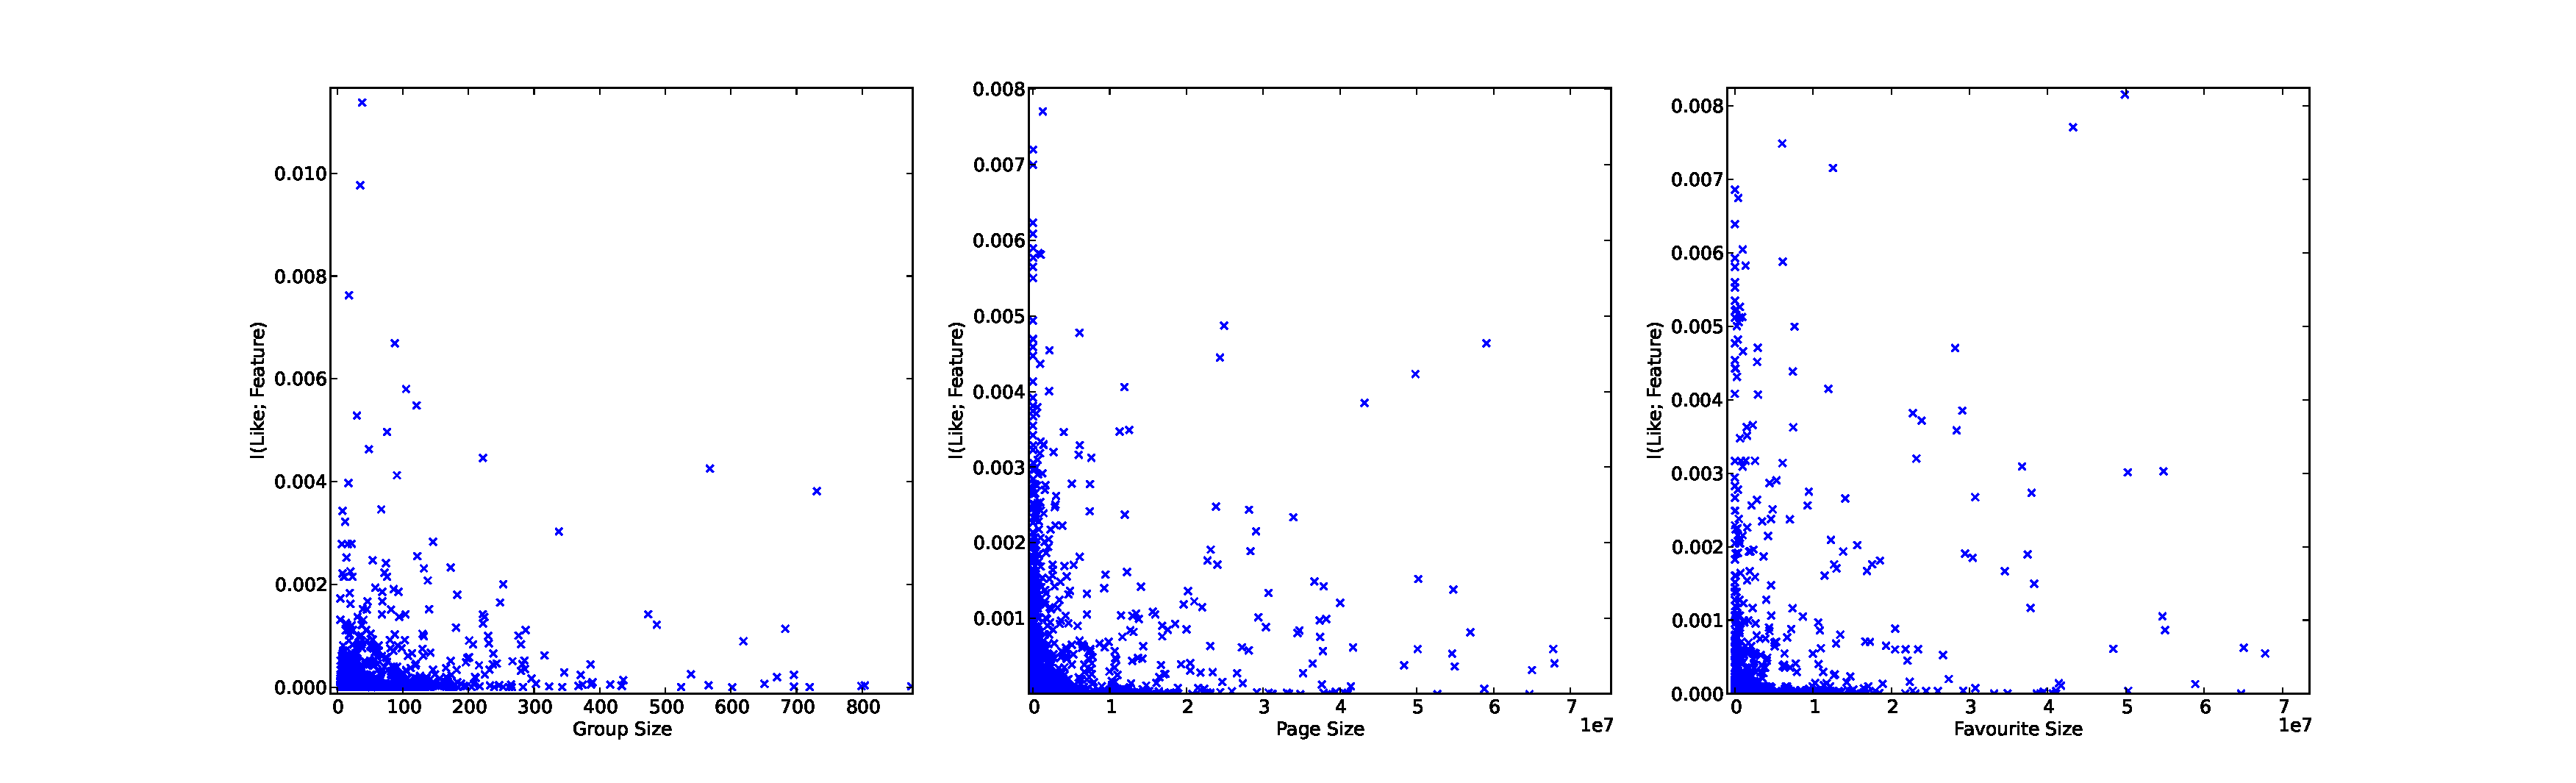
\includegraphics[width=100mm, height=30mm]{data/MIvsSize.eps}
\caption {Mutual Information vs Size}
\label {Fig: Mutual Information vs Size}
\end{figure}

\begin{figure}
\centering
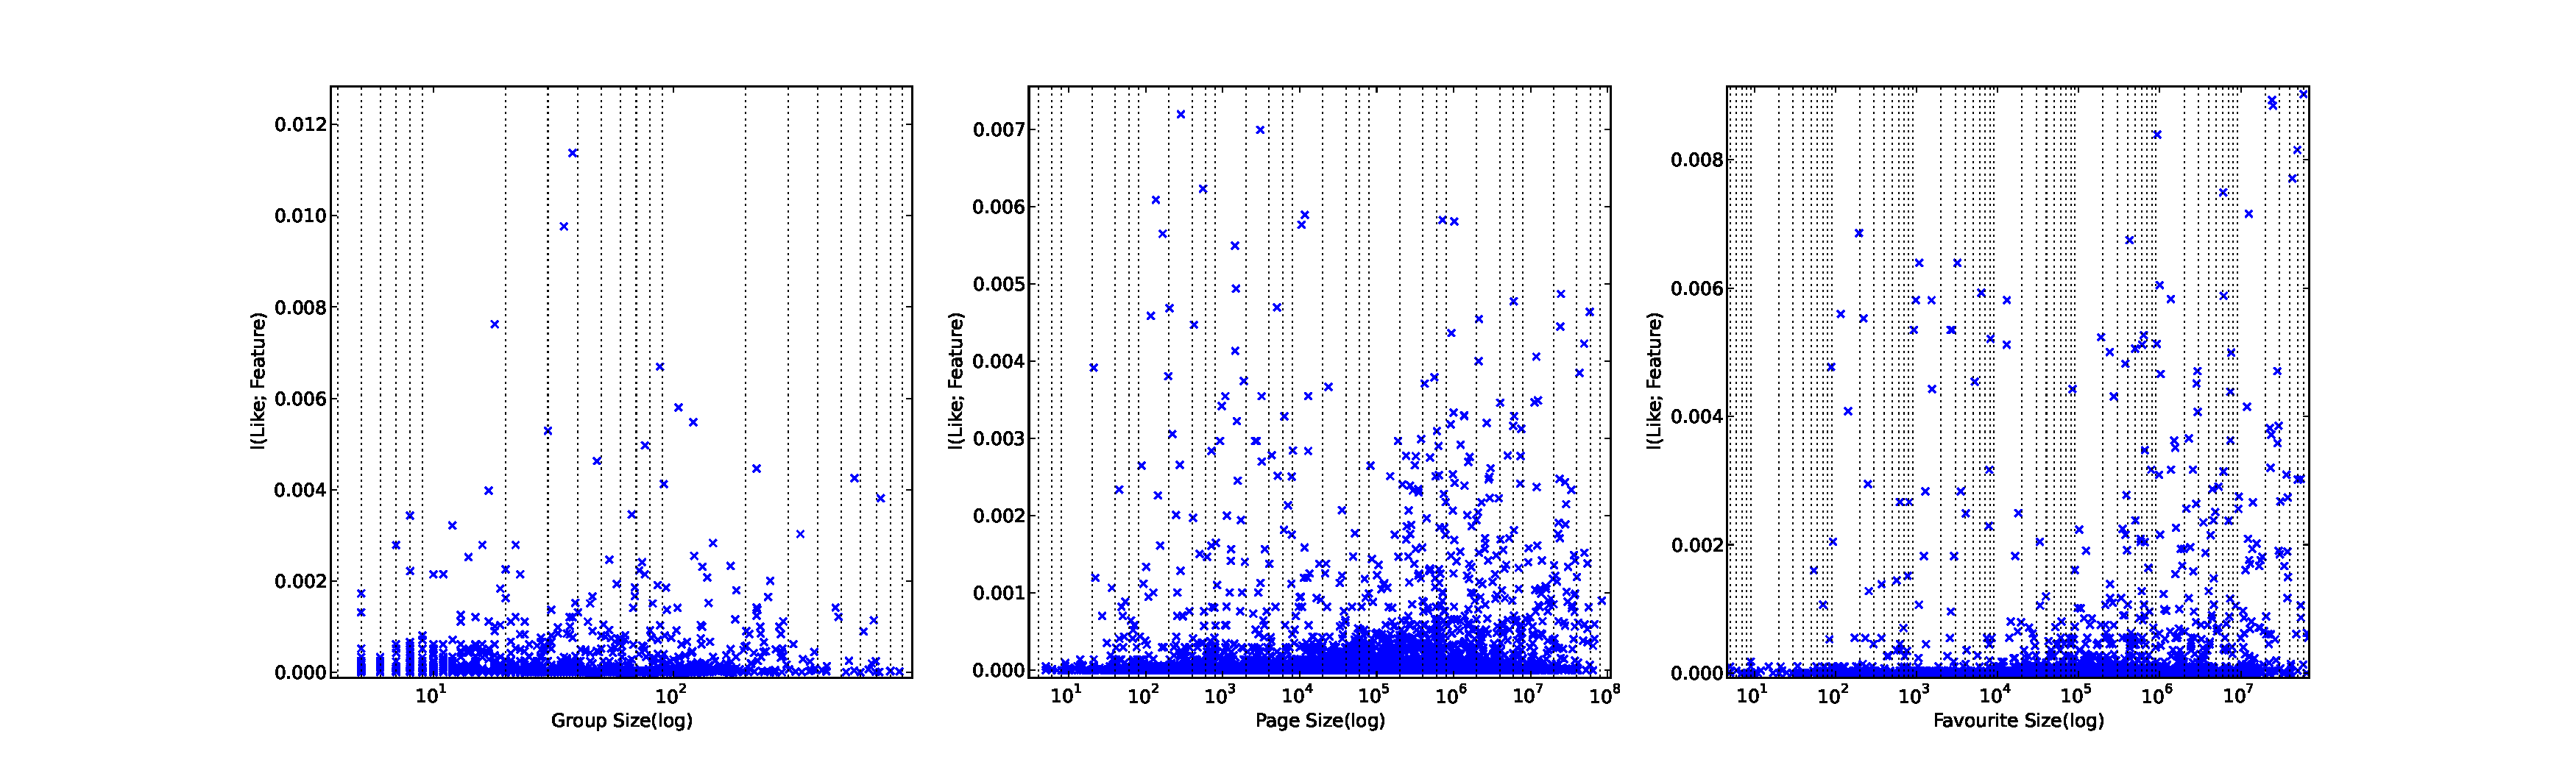
\includegraphics[width=100mm, height=30mm]{data/MIvsSizelog.eps}
\caption{Mutual Information  vs Size(log)}
\label {Fig: Mutual Information vs Size(log)}
\end{figure}


\cleardoublepage
\begin{table}
	\centering
	\begin{tabular}{| >{\small}l | >{\small}r | >{\small}r | >{\small}r | >{\small}r | >{\small}r |}
		\hline
		Modality & ConditionalEntropy & (Like,True) & (Dislike,True) & (Like,False) & (Dislike,False)\\
		\hline
		\textbf{video} & 0.850116919421 & 117 & 44 & 2402 & 2962\\
		\hline
		\textbf{link} & 0.914700608855 & 989 & 486 & 1530 & 2520\\
		\hline
		\textbf{post} & 0.918160390299 & 1154 & 576 & 1365 & 2430\\
		\hline
		\textbf{photo} & 0.9259513318 & 675 & 349 & 1844 & 2657\\
		\hline
		\hline
		\textbf{Modality} & MutualInformation & (Like,True) & (Dislike,True) & (Like,False) & (Dislike,False)\\
		\hline
		\textbf{post} & 0.0594688018722 & 1154 & 576 & 1365 & 2430\\
		\hline
		\textbf{link} & 0.0490133947836 & 989 & 486 & 1530 & 2520\\
		\hline
		\textbf{photo} & 0.0273700186713 & 675 & 349 & 1844 & 2657\\
		\hline
		\textbf{video} & 0.0064494273283 & 117 & 44 & 2402 & 2962\\
		\hline
		\hline
		\textbf{Type}  & Conditional Entropy & (Like,True) & (Dislike,True) & (Like,False) & (Dislike,False)\\
		\hline
		\textbf{Tags}  &  0.919971597996 & 809 & 407 & 1710 & 2599\\
		\hline
		\textbf{Comments}  &  0.921373670369 & 1009 & 511 & 1510 & 2495\\
		\hline
		\textbf{Likes}  &  0.924414408934 & 1135 & 583 & 1384 & 2423\\
		\hline
		\textbf{Type}  & Mutual Information & (Like,True) & (Dislike,True) & (Like,False) & (Dislike,False)\\
		\hline
		\textbf{Likes}  &  0.0553328447681 & 1135 & 583 & 1384 & 2423\\
		\hline
		\textbf{Comments}  &  0.0479360954681 & 1009 & 511 & 1510 & 2495\\
		\hline
		\textbf{Tags}  &  0.0361031572103 & 809 & 407 & 1710 & 2599\\
		\hline
		\textbf{Direction} & Mutual Information & (Like,True) & (Dislike,True) & (Like,False) & (Dislike,False)\\
		\hline
		\textbf{Outgoing}  &  0.049470651248 & 1074 & 562 & 1445 & 2444\\
		\hline
		\textbf{Incoming}  &  0.0470981200647 & 1081 & 584 & 1438 & 2422\\
		\hline
		\textbf{Direction} & Conditional Entropy &  (Like,True) & (Dislike,True) & (Like,False) & (Dislike,False)\\
		\hline
		\textbf{Outgoing}  &  0.928353525673 & 1074 & 562 & 1445 & 2444\\
		\hline
		\textbf{Incoming}  &  0.934921690705 & 1081 & 584 & 1438 & 2422\\
		\hline
		
	\end{tabular}
\end{table}

\begin{table}
	\centering
	\begin{tabular}{| >{\small}l | >{\small}r | >{\small}r | >{\small}r | >{\small}r | >{\small}r |}
	\hline
	Interaction & Conditional Entropy & (Like,True) & (Dislike,True) & (Like,False) & (Dislike,False)\\
	\hline
	\textbf{VIDEO\_LIKES\_OUTGOING} & 0.722397472066 & 31 & 7 & 2488 & 2999\\
	\hline
	\textbf{VIDEO\_LIKES\_INCOMING} & 0.775086171837 & 43 & 12 & 2476 & 2994\\
	\hline
	\textbf{POST\_TAGS\_INCOMING} & 0.802855788214 & 444 & 143 & 2075 & 2863\\
	\hline
	\textbf{PHOTO\_COMMENTS\_OUTGOING} & 0.816036600382 & 135 & 45 & 2384 & 2961\\
	\hline
	\textbf{PHOTO\_TAGS\_OUTGOING} & 0.818540125915 & 427 & 145 & 2092 & 2861\\
	\hline
	\textbf{PHOTO\_LIKES\_INCOMING} & 0.853009353418 & 277 & 106 & 2242 & 2900\\
	\hline
	\textbf{LINK\_LIKES\_OUTGOING} & 0.855368864256 & 728 & 282 & 1791 & 2724\\
	\hline
	\textbf{POST\_TAGS\_OUTGOING} & 0.856163233945 & 505 & 196 & 2014 & 2810\\
	\hline
	\textbf{LINK\_COMMENTS\_INCOMING} & 0.865533720447 & 530 & 213 & 1989 & 2793\\
	\hline
	\textbf{POST\_LIKES\_OUTGOING} & 0.870618130159 & 834 & 342 & 1685 & 2664\\
	\hline
	\textbf{VIDEO\_COMMENTS\_OUTGOING} & 0.883596675997 & 43 & 18 & 2476 & 2988\\
	\hline
	\textbf{LINK\_LIKES\_INCOMING} & 0.888406184542 & 742 & 326 & 1777 & 2680\\
	\hline
	\textbf{POST\_LIKES\_INCOMING} & 0.889444522106 & 929 & 410 & 1590 & 2596\\
	\hline
	\textbf{POST\_COMMENTS\_INCOMING} & 0.890449138325 & 763 & 338 & 1756 & 2668\\
	\hline
	\textbf{PHOTO\_TAGS\_INCOMING} & 0.890856994354 & 485 & 215 & 2034 & 2791\\
	\hline
	\textbf{POST\_COMMENTS\_OUTGOING} & 0.894129257133 & 694 & 312 & 1825 & 2694\\
	\hline
	\textbf{LINK\_COMMENTS\_OUTGOING} & 0.895134128697 & 543 & 245 & 1976 & 2761\\
	\hline
	\textbf{PHOTO\_LIKES\_OUTGOING} & 0.89759612767 & 161 & 73 & 2358 & 2933\\
	\hline
	\textbf{PHOTO\_COMMENTS\_INCOMING} & 0.906541518549 & 290 & 137 & 2229 & 2869\\
	\hline
	\textbf{VIDEO\_COMMENTS\_INCOMING} & 0.92652449307 & 53 & 27 & 2466 & 2979\\
	\hline
	\textbf{FRIENDS} & 0.965942963751 & 1392 & 895 & 1127 & 2111\\
	\hline
	\textbf{VIDEO\_TAGS\_INCOMING} & 0.999999611934 & 17 & 17 & 2502 & 2989\\
	\hline
	\textbf{VIDEO\_TAGS\_OUTGOING} & 0.999999611934 & 16 & 16 & 2503 & 2990\\
	\hline
	\end{tabular}
\end{table}

\cleardoublepage

\begin{table}
	\centering
	\begin{tabular}{| >{\small}l | >{\small}r | >{\small}r | >{\small}r | >{\small}r | >{\small}r |}
	\hline
	Interaction & Mutual Information & (Like,True) & (Dislike,True) & (Like,False) & (Dislike,False)\\
	\hline
	\textbf{POST\_LIKES\_INCOMING} & 0.0524561740233 & 929 & 410 & 1590 & 2596\\
	\hline
	\textbf{POST\_LIKES\_OUTGOING}& 0.050407410911 & 834 & 342 & 1685 & 2664\\
	\hline
	\textbf{FRIENDS} & 0.0473539909731 & 1392 & 895 & 1127 & 2111\\
	\hline
	\textbf{LINK\_LIKES\_OUTGOING}& 0.0457244144031 & 728 & 282 & 1791 & 2724\\
	\hline
	\textbf{POST\_COMMENTS\_INCOMING}& 0.0405155210996 & 763 & 338 & 1756 & 2668\\
	\hline
	\textbf{LINK\_LIKES\_INCOMING}& 0.0396004717225 & 742 & 326 & 1777 & 2680\\
	\hline
	\textbf{POST\_COMMENTS\_OUTGOING}& 0.0352609340207 & 694 & 312 & 1825 & 2694\\
	\hline
	\textbf{POST\_TAGS\_INCOMING}& 0.0315770377754 & 444 & 143 & 2075 & 2863\\
	\hline
	\textbf{LINK\_COMMENTS\_INCOMING}& 0.0299391900579 & 530 & 213 & 1989 & 2793\\
	\hline
	\textbf{POST\_TAGS\_OUTGOING}& 0.0296108833783 & 505 & 196 & 2014 & 2810\\
	\hline
	\textbf{PHOTO\_TAGS\_OUTGOING}& 0.0286060075004 & 427 & 145 & 2092 & 2861\\
	\hline
	\textbf{LINK\_COMMENTS\_OUTGOING}& 0.0261662648974 & 543 & 245 & 1976 & 2761\\
	\hline
	\textbf{PHOTO\_TAGS\_INCOMING}& 0.0235803030398 & 485 & 215 & 2034 & 2791\\
	\hline
	\textbf{PHOTO\_LIKES\_INCOMING}& 0.0155060725343 & 277 & 106 & 2242 & 2900\\
	\hline
	\textbf{PHOTO\_COMMENTS\_INCOMING}& 0.0120447345005 & 290 & 137 & 2229 & 2869\\
	\hline
	\textbf{PHOTO\_COMMENTS\_OUTGOING}& 0.00851951888057 & 135 & 45 & 2384 & 2961\\
	\hline
	\textbf{PHOTO\_LIKES\_OUTGOING}& 0.00687365820792 & 161 & 73 & 2358 & 2933\\
	\hline
	\textbf{VIDEO\_LIKES\_INCOMING}& 0.00309679794205 & 43 & 12 & 2476 & 2994\\
	\hline
	\textbf{VIDEO\_LIKES\_OUTGOING}& 0.00259896191026 & 31 & 7 & 2488 & 2999\\
	\hline
	\textbf{VIDEO\_COMMENTS\_OUTGOING}& 0.00197259388552 & 43 & 18 & 2476 & 2988\\
	\hline
	\textbf{VIDEO\_COMMENTS\_INCOMING}& 0.0017837362825 & 53 & 27 & 2466 & 2979\\
	\hline
	\textbf{VIDEO\_TAGS\_INCOMING}& 3.598735115e-05 & 17 & 17 & 2502 & 2989\\
	\hline
	\textbf{VIDEO\_TAGS\_OUTGOING}& 3.39757297236e-05 & 16 & 16 & 2503 & 2990\\
	\hline
	\end{tabular}
\end{table}

	

\input affinity_filtering

\input interaction_analysis

\input activity_analysis

\section{Related Work}

%\input related-work

\section{Conclusions}

%\input conclusions

\bibliography{bibliography}
\bibliographystyle{aaai}

\end{document}

